\documentclass[a4]{beamer}
\usepackage{amssymb}
\usepackage{graphicx}
\usepackage{subfigure}
\usepackage{newlfont}
\usepackage{amsmath,amsthm,amsfonts}
%\usepackage{beamerthemesplit}
\usepackage{pgf,pgfarrows,pgfnodes,pgfautomata,pgfheaps,pgfshade}
\usepackage{mathptmx} % Font Family
\usepackage{helvet} % Font Family
\usepackage{color}
\mode<presentation> {
	\usetheme{Default} % was Frankfurt
	\useinnertheme{rounded}
	\useoutertheme{infolines}
	\usefonttheme{serif}
	%\usecolortheme{wolverine}
	% \usecolortheme{rose}
	\usefonttheme{structurebold}
}
\setbeamercovered{dynamic}
\title[MA4413]{Statistics for Computing \\ {\normalsize MA4413 Lecture 11A}}
\author[Kevin O'Brien]{Kevin O'Brien \\ {\scriptsize kevin.obrien@ul.ie}}
\date{Autumn 2011}
%\institute[Maths \& Stats]{Dept. of Mathematics \& Statistics, \\ University \textit{of} Limerick}
\renewcommand{\arraystretch}{1.5}
%------------------------------------------------------------------------%

\begin{document}


\begin{frame} \frametitle{Discrete Memoryless Channels}
%\textbf{A. Channel Representation:}\\
\begin{itemize}
	\item A communication channel is the path or medium through which the symbols flow to the receiver. \item A discrete memoryless channel (DMC) is a statistical model with an input X and an output Y.
	During each unit of the time, the channel accepts an input symbol from X, and in
	response it generates an output symbol from Y. \item  The channel is ``discrete" when the alphabets of X and
	Y are both finite.\item It is ``memoryless" when the current output depends on only the current input and
	not on any of the previous inputs.\end{itemize}
\end{frame}



%\end{document}

\begin{frame} \frametitle{DISCRETE MEMORYLESS CHANNELS}
\textbf{A. Channel Representation:}\\
\begin{itemize}
	\item A communication channel is the path or medium through which the symbols flow to the receiver. \item A discrete memoryless channel (DMC) is a statistical model with an input X and an output Y.
	During each unit ofthe time (signaling interval), the channel accepts an input symbol from X, and iu
	response it generates an output symbol from Y.\item  The channel is "discrete" when the alphabets of X and
	Y are both finite.\item It is ``memoryless" when the current output depends on only the current input and
	not on any of the previous inputs.\end{itemize}
\end{frame}
%r. - · yi
%XI: X Ptytnt ykzyr
%rn,. · yn

\begin{frame}
\frametitle{Discrete memoryless channel - FIX THIS}
\begin{itemize}
	\item A diagram of a DMC with nt inputs and n outputs is illustrated in Fig. l0-1. The input X consists
	of input symbols ir, , X2,   xm. 
	\item The a priori probabilities of these source symbols P(.x,) are assumed to be known. 
	\item The output $Y$ consists of output symbols $\{y_1,y_2,\ldots, y_i \}$
	
	\item Each possible input-to-output path is indicated along with a conditional probability $P(y_i|x_i)$, where $P(y_i|x_i)$  is the conditional probability of
	obtaining output $y_i$ given that the input is $x_i$, and is called a \textbf{\emph{channel transition probability}}.
\end{itemize}

\end{frame}

\begin{frame}
\frametitle{Channel Matrix - FIX THIS}

A channel is completely specified by the complete set of transition probabilities. Accordingly, the
channel of Fig. 10-l is ol` ten speciiied by the matrix of transition probabilities [P(YlX)l, given by
%P<yilxi> P<yc|Xt>   !’<ytl¤<i>
%W YIXM = P(yllXz> Plyzlxs)   i’<yiI~¤s> (NUI)
%/’<yi|xm) P<ysI·rm>   P<ytI><ml

The matrix [P(YlX)] is called thc channel matrix. Since each input to the channel results in some
output, each row of the channel matrix niust snm to unity. that is,
%ZP(yylx;) : l lor all 1 (10.12)
\end{frame}


\begin{frame}
\frametitle{Discrete memoryless channel}
\begin{itemize}
	\item A DMC can have any number of inputs and any number of outputs.
	\item For a DMC with ``m" inputs and ``n" outputs, the input X consists of input symbols $x_1, x_2, \ldots x_m$.
	\item The probabilities of these source symbols $P(x_i)$ are assumed to be known.
	\item The output Y consists of output symbols $\{y_1,y_2,\ldots, y_n \}$
	\item Each possible input-to-output path is indicated along with a conditional probability $P(y_i|x_i)$, where $P(y_i|x_i)$  is the conditional probability of
	obtaining output $y_i$ given that the input is $x_i$. \item $P(y_i|x_i)$ is called a \textbf{\emph{channel transition probability}}.
\end{itemize}
\end{frame}
%\end{document}
%--------------------------------------------------------%
%--------------------------------------------------------%
\begin{frame}
\frametitle{Discrete memoryless channel}
\begin{itemize}
\item On the next slide, we present a binary DMC, with the channel transition probabilities indicated.
\item $P(Y_1|X_1)$ = 0.9  and $P(Y_2|X_1)$ = 0.1
\item $P(Y_1|X_2)$ = 0.2  and $P(Y_2|X_2)$ = 0.8
\end{itemize}
\end{frame}

\frame{
\frametitle{Discrete Memoryless Channels}

\begin{center}
\includegraphics[scale=0.54]{images/10Bnet2}
\end{center}

}

%\frame{
%\frametitle{Discrete Memoryless Channels}
%
%\begin{center}
%\includegraphics[scale=0.54]{10Bnet2}
%\end{center}
%}
%- Data Compression ( www.datacompression.com )

\begin{frame}
\frametitle{Channel Matrix}

A channel is completely specified by the complete set of transition probabilities. Accordingly, a
channel is specified by the matrix of transition probabilities $[P(YlX)]$, given by

\[  [P(Y|X)]  = \left[ \begin{array}{cccc}
P(y_1|x_1) & P(y_2|x_1) & \ldots & P(y_n|x_1) \\
P(y_1|x_2) & P(y_2|x_2) & \ldots & P(y_n|x_2) \\
\ldots & \ldots & \ldots & \ldots \\
P(y_1|x_m) & P(y_2|x_m) & \ldots & P(y_n|x_n) \\
\end{array} \right] \]


The matrix $[P(YlX)]$ is called the \textbf{\emph{channel matrix}}.
%ZP(yylx;) : l lor all 1 (10.12)
\end{frame}

\begin{frame}
\frametitle{Channel Matrix}
\begin{itemize}
\item Since each input to the channel results in some
output, each row of the channel matrix must sum to unity (i.e. all rows must add up to 1. This condition is not necessary for columns).
\item For the binary DMC presented previously, the channel matrix is
\[  [P(Y|X)]  = \left[ \begin{array}{cc}
0.9 & 0.1  \\
0.2 & 0.8 \\
\end{array} \right] \]
\item (Remark: This is not a binary symmetric channel)
\end{itemize}
\end{frame}


\begin{frame}
\frametitle{Channel Matrix}
\begin{itemize}
\item The input probabilities $P(X)$ are represented by the row matrix
\[  [P(X)]  = \left[ \begin{array}{cccc}
P(x_1) & P(x_2) & \ldots & P(x_m) \\
\end{array} \right] \]
\item The input probabilities $P(Y)$ are represented by the row matrix
\[  [P(Y)]  = \left[ \begin{array}{cccc}
P(y_1) & P(y_2) & \ldots & P(y_n) \\
\end{array} \right] \]
\item We can compute $[P(Y)] $ by the following formula: $[P(Y)]  = [P(X)]\times [P(Y|X)]$
\item (Note: Be mindful of the dimensions of each matrix).
\end{itemize}
\end{frame}

\begin{frame}
\frametitle{Channel Matrix}
\begin{itemize}
\item Suppose for our Binary DMC that the input probabilities were given by $[P(X)] = [ 0.5\mbox{   }0.5]$.
\item Compute $[P(Y)]$, given the channel matrix given in previous slides.
\[  [P(Y)]  =  \left[ \begin{array}{cc}
0.5 & 0.5 \\
\end{array} \right] \times \left[ \begin{array}{cc}
0.9 & 0.1  \\
0.2 & 0.8 \\
\end{array} \right] \]

\item Solving
\[  [P(Y)]  =  \left[ \begin{array}{cc}
(0.5 \times 0.9)+(0.5 \times 0.2) & (0.5 \times 0.1)+(0.5 \times 0.8) \\
\end{array} \right]  \]

\item Simplifying \[  [P(Y)]  =  \left[ \begin{array}{cc}
0.55 & 0.45 \\
\end{array} \right]  \]
\end{itemize}
\end{frame}


\begin{frame}
\frametitle{Channel Matrix}
\begin{itemize}
\item Let $[P(X)]$ is presented as a diagonal matrix , i.e.

\[  [P(X)]_d  = \left[ \begin{array}{cccc}
P(x_1) &0 & \ldots & 0 \\
0 & P(x_2)& \ldots & 0 \\
\ldots & \ldots & \ldots & \ldots \\
0& 0 & \ldots & P(x_m) \\
\end{array} \right] \]
\item The \emph{\textbf{ joint probability matrix}} $[P(X,Y)]$can be computed as
$[P(X,Y)]  = [P(X)]_d\times [P(Y|X)]$
\end{itemize}
\end{frame}

\begin{frame}
\frametitle{Channel Matrix}
\begin{itemize}
\item For the Binary DMC described in the previous example, compute the joint probability matrix.
\item Diagonalize the input probabilities for $X$.
\[  [P(X)]_d  = \left[ \begin{array}{cc}
0.5 & 0.0  \\
0.0 & 0.5\\
\end{array} \right] \]

\item Simplifying
\[  [P(X,Y)]  =  \left[ \begin{array}{cc}
(0.5 \times 0.9)+(0 \times 0.2) & (0.5 \times 0.1)+(0 \times 0.8) \\
(0 \times 0.9)+(0.5 \times 0.2) & (0 \times 0.1)+(0.5 \times 0.8) \\
\end{array} \right]  \]


\item Solving
\[  [P(X,Y)]  =  \left[ \begin{array}{cc}
0.45 & 0.05 \\
0.1  & 0.4 \\
\end{array} \right]  \]
\end{itemize}
Notice the row and column totals.
\end{frame}

%--------------------------------------------------------%

\frame{
	\frametitle{Discrete Memoryless Channels}
	
	\begin{center}
		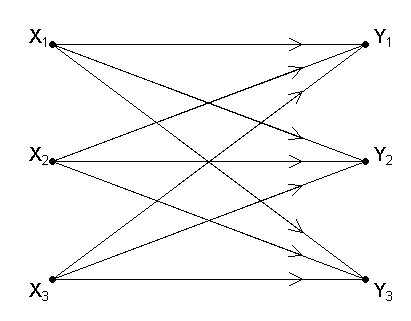
\includegraphics[scale=0.54]{images/10Bnet}
	\end{center}
	
}

\end{document}